\documentclass[9pt]{beamer}
% Created By Gouthaman KG
%~~~~~~~~~~~~~~~~~~~~~~~~~~~~~~~~~~~~~~~~~~~~~~~~~~~~~~~~~~~~~~~~~~~~~~~~~~~~~~
% Use roboto Font (recommended)
\usepackage[sfdefault]{roboto}
\usepackage[utf8]{inputenc}
\usepackage[T1]{fontenc}
%~~~~~~~~~~~~~~~~~~~~~~~~~~~~~~~~~~~~~~~~~~~~~~~~~~~~~~~~~~~~~~~~~~~~~~~~~~~~~~

%~~~~~~~~~~~~~~~~~~~~~~~~~~~~~~~~~~~~~~~~~~~~~~~~~~~~~~~~~~~~~~~~~~~~~~~~~~~~~~
% Define where theme files are located. ('/styles')
\usepackage{styles/fluxmacros}
\usefolder{styles}
% Use Flux theme v0.1 beta
% Available style: asphalt, blue, red, green, gray
\usetheme[style=asphalt]{flux}
%~~~~~~~~~~~~~~~~~~~~~~~~~~~~~~~~~~~~~~~~~~~~~~~~~~~~~~~~~~~~~~~~~~~~~~~~~~~~~~

%~~~~~~~~~~~~~~~~~~~~~~~~~~~~~~~~~~~~~~~~~~~~~~~~~~~~~~~~~~~~~~~~~~~~~~~~~~~~~~
% Extra packages for the demo:
\usepackage{booktabs}
\usepackage{multirow}
\usepackage{colortbl}
\usepackage{ragged2e}
\usepackage{schemabloc}
\usepackage{hyperref}
\hypersetup{
    colorlinks=true,
    urlcolor=purple,
    linkcolor=.
}

\usepackage{caption,subcaption}
\usebackgroundtemplate{

\includegraphics[width=\paperwidth,height=\paperheight]{images/background.jpg}}
\setbeamertemplate{caption}[numbered]

% Informations
\title{Project presentation}
\subtitle{Applying tabu search to the capacitated vehicle routing problem}

\author{Phan Ngoc Lan}
\institute{Hanoi University of Science and Technology}
\titlegraphic{images/hust.png} %change this to your preferred logo or image(the image is located on the top right corner).
%~~~~~~~~~~~~~~~~~~~~~~~~~~~~~~~~~~~~~~~~~~~~~~~~~~~~~~~~~~~~~~~~~~~~~~~~~~~~~~

\begin{document}
\AtBeginSection[]{
    \begin{frame}<beamer>
        \frametitle{Outline}
        \tableofcontents[currentsection]
    \end{frame}
}

% Generate title page
\titlepage

\begin{frame}
 \frametitle{Table of contents}
 \tableofcontents
\end{frame}

\section{The capacitated vehicle routing problem}
\begin{frame}{Vehicle routing problems}
\begin{block}{}
    What is the optimal set of routes for a fleet of vehicles to traverse in order to deliver to a given set of customers?
\end{block}

Proposed by Dantzig and Ramser \cite{dantzig1959truck}, vehicle routing problems (VRP) occur naturally in multiple fields, most notably transportation and logistics.

There are many variants of the VRP:
\begin{itemize}
    \item Capacitated Vehicle Routing Problem (CVRP)
    \item Vehicle Routing Problem with Time Windows (VRPTW)
    \item Vehicle Routing Problem with Profits (VRPP)
    \item etc,\dots
\end{itemize}
\end{frame}

\begin{frame}{Capacitated vehicle routing}
The capacitated vehicle routing problem (CVRP) is one of the most basic and well-studied variants of VRP.

Each customer has a demand index that needs to be fulfilled. Each vehicle has a capacity for service. A vehicle cannot satisfy demands exceeding its capacity.
\end{frame}

\begin{frame}{Mathematical formulation}
The mathematical formulation for CVRP is modified from TSP:

\begin{equation}
    min \sum_{i \in V} \sum_{j \in V} c_{ij}x_{ij}
\end{equation}
subject to
\begin{align}
    \sum_{i \in V} x_{ij} & = 1 \ \forall j \in V \backslash \{0\} \\
    \sum_{j \in V} x_{ij} & = 1 \ \forall i \in V \backslash \{0\} \\
    \sum_{i \in V} x_{i0} & = K \\
    \sum_{j \in V} x_{0j} & = K \\
    \sum_{i \notin S} \sum_{j \in S} x_{ij} & \geq r(S), \forall S \subseteq V \backslash \{0\},\ S \neq \emptyset\\
    x_{ij} & \in \{ 0, 1 \} \forall i,j \in V
\end{align}

\end{frame}

\section{Related works}
\begin{frame}{Related works}
Christofides et al. \cite{christofides1976vehicle} reviewed a number of methods for solving VRP, and presented 3 datasets for the problem.

Reimann et al. \cite{reimann2004d} propsed an ACO-based method for large-scale VRPs

Pisinger et al. \cite{pisinger2007general} proposed a large neighborhood search method (ALNS) for solving a variety of VRP problems (including CVRP, VRPTW, etc). Different problem types are transformed into the Rich Pickup and Delivery Problem with Time Windows. The search is adaptive, where each iteration selects a "destroy" neighborhood and a "repair" neighborhood to advance the current solution.

Prins et al. \cite{prins2009grasp} proposed $GRASP \times ELS$, a hybrid between the GRASP framework (consisting of multiple restarts and search with mutations) and evolutionary local search (ELS).
\end{frame}

\section{Tabu search}
\begin{frame}{Overview}
Tabu search \cite{glover1986future} is a local search paradigm that uses memory structures to prevent the search from visiting previous solutions.

Proposed by Glover and Hansen in 1986.

Full tabu search includes 3 phases:
\begin{itemize}
    \item Short-term: Search using tabu list starting from the initial solution
    \item Intensification: A good solution is selected and the search focuses on this solution's neighborhood
    \item Diversification: The search explores a different area in the search space to find better solutions
\end{itemize}
\end{frame}

\begin{frame}{SimpleTabu for CVRP}
    SimpleTabu: A full tabu search to solve CVRP.

    \begin{enumerate}
        \item \textbf{Initialization}: initializes a solution and long-term memory structures
        \item \textbf{Short-term phase}: runs the search with tabu constraints. Updates the elite set and frequency matrix at each iteration
        \item \textbf{Intensification phase}: selects a solution in the elite set as the initial solution. Runs the search with tabu constraints. Updates the elite set and frequency matrix at each iteration
        \item \textbf{Diversification phase}: generates a diversified solution using the frequency matrix. Runs the search with tabu constraints. Updates the elite set and frequency matrix at each iteration
    \end{enumerate}
\end{frame}

\begin{frame}{SimpleTabu - Initialization}
    The initial solution is generated using the Clarke-Wright greedy algorithm (savings algorithm). Each edge $(i, j)$ is assigned a savings value, which is the amount of cost that can be saved by joining the routes $0, i, 0$ and $0, j, 0$. Edges are then greedily joined from the highest weighted edge to the lowest.

    The savings algorithm is deterministic. To add randomness, we can shuffle the savings list or assign random weights to each edge's savings value.

    SimpleTabu creates the initial solution by randomizing the Clarke-Wright algorithm.
\end{frame}

\begin{frame}{SimpleTabu - Exploration}
    Many exploration operators have been proposed for the CVRP:

    \begin{itemize}
        \item Relocate: Move a location on a single route
        \item 2-opt*: Swap two locations on two different routes
        \item Or-opt: Attach a random segment from one route to another route
        \item Cross-exchange: Swaps two pairs of locations on two different routes
        \item etc,\dots
    \end{itemize}

    SimpleTabu uses Relocate, 2-opt* and Or-opt.
\end{frame}

\begin{frame}{SimpleTabu - Exploration}
    \begin{figure}[ht]
        \centering
        \begin{subfigure}[b]{\linewidth}
            \centering
            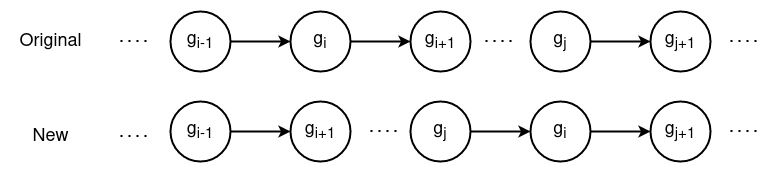
\includegraphics[width=0.7\textwidth]{images/lsops-relocate.png}
            \caption{Relocate}
        \end{subfigure}
        \begin{subfigure}[b]{0.35\linewidth}
            \centering
            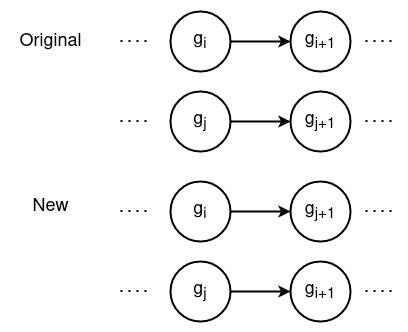
\includegraphics[width=0.95\textwidth]{images/lsops-2-opt.png}
            \caption{2-opt*}
        \end{subfigure}
        \begin{subfigure}[b]{0.63\linewidth}
            \centering
            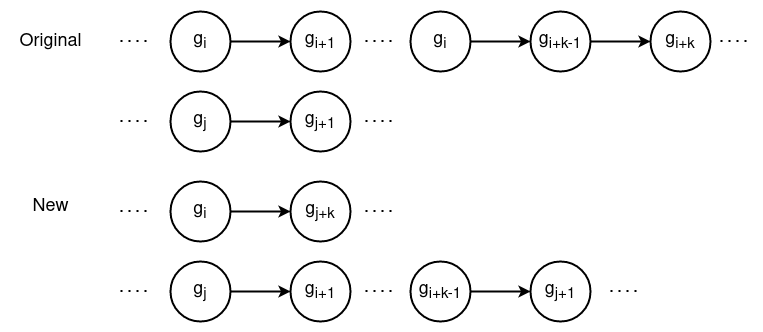
\includegraphics[width=0.95\textwidth]{images/lsops-or-opt.png}
            \caption{Or-opt}
        \end{subfigure}
        \caption{Visualizations of local search operators used by SimpleTabu \footnote{Figures based on \cite{mcnabb2015testing}}}
    \end{figure}
\end{frame}

\begin{frame}{SimpleTabu - Intensification}
Each time a solution outperforms the current best solution, it is added to the elite set.

The intensification phase selects a random solution in the elite set to begin the search.

Goal: further explore the area adjacent to a good solution in order to find improvements.
\end{frame}

\begin{frame}{SimpleTabu - Diversification}
At each iteration, an edge-frequency matrix $F$ is updated by incrementing the count of each edge that appears in the current solution. Frequently used edges have higher weights.

Before diversification, SimpleTabu generates an inverse weight matrix $IW$, where:
\begin{equation*}
    IW_{ij} = 1 - \frac{F_{ij}}{\sum F}
\end{equation*}

$IW$ is used as the savings weight for the Clarke-Wright algorithm, which creates the initial solution for diversification.

\end{frame}

\section{Experiments}
\begin{frame}{Experiment settings}
2 experiments are performed:
\begin{enumerate}
    \item Ablation study: 4 variations of SimpleTabu with different operators are compared
    \item Comparison: SimpleTabu is compared with ALNS (large neighborhood search) and GRELS (GRASPxELS)
\end{enumerate}

All experiments use the Christofides et al. 1979 dataset. Includes 14 instances of medium size.

Results for \href{http://www.vrp-rep.org/references/item/pisinger-and-ropke-2007.html}{ALNS} and \href{http://www.vrp-rep.org/references/item/prins-2009.html}{GRELS} are reported at VRP-REP.

SimpleTabu is implemented in Python3. Experiments are run using the PyPy \cite{rigo2006pypy} runtime on a 2-core AMD EPYC 2.2Ghz CPU with 4GB RAM.
\end{frame}

\begin{frame}{Algorithm parameters}
    \begin{table}[htp]
\centering
\begin{tabular}{|l|r|}
    \hline
    \multicolumn{1}{|c|}{\textbf{Parameter}} & \multicolumn{1}{c|}{\textbf{Value}} \\ \hline
    Short-term max iters. & 300 \\ \hline
    Short-term early-stop tolerance & 10 \\ \hline
    Short-term tabu list size & 300 \\ \hline
    Intensification max iters. & 300 \\ \hline
    Intensification early-stop tolerance & 5 \\ \hline
    Intensification tabu list size & 200 \\ \hline
    Diversification max iters. & 300 \\ \hline
    Diversification early-stop tolerance & 20 \\ \hline
    Diversification tabu list size & 400 \\ \hline
    Candidate set size & 3000 \\ \hline
    Elite set size & 10 \\ \hline
\end{tabular}
\caption{Parameter values for SimpleTabu}
\label{tab:tabu-params}
\end{table}

\end{frame}

\begin{frame}{Ablation study - Results}
\begin{table}[]
\resizebox{\textwidth}{!}{
\begin{tabular}{ |c|r|r|r|r|r|r|r|r| }
\hline
\multicolumn{1}{|c|}{ \multirow{2}{*}{ \textbf{ Instance } } } & \multicolumn{2}{|c|}{ \textbf{ SimpleTabu (Full) } } & \multicolumn{2}{|c|}{ \textbf{ SimpleTabu (No Or-Opt) } } & \multicolumn{2}{|c|}{ \textbf{ SimpleTabu (No 2-Opt*) } } & \multicolumn{2}{|c|}{ \textbf{ SimpleTabu (No Relocate) } } \\
\cline{ 2-9 }
 & \multicolumn{1}{|c|}{ Best } & \multicolumn{1}{|c|}{ Std } & \multicolumn{1}{|c|}{ Best } & \multicolumn{1}{|c|}{ Std } & \multicolumn{1}{|c|}{ Best } & \multicolumn{1}{|c|}{ Std } & \multicolumn{1}{|c|}{ Best } & \multicolumn{1}{|c|}{ Std } \\ \hline
CMT01 &  581.02 & 10.84 & \textbf{ 570.24 } & 17.04 &  593.18 & \textbf{ 8.23 } &  595.83 & 53.00 \\ \hline
CMT02 & \textbf{ 900.68 } & 17.59 &  911.27 & 16.73 &  934.70 & \textbf{ 12.35 } &  960.40 & 32.64 \\ \hline
CMT03 &  918.25 & \textbf{ 7.61 } & \textbf{ 905.49 } & 29.29 &  912.26 & 18.47 &  952.33 & 27.77 \\ \hline
CMT04 &  1186.45 & 29.41 &  1215.15 & \textbf{ 15.07 } & \textbf{ 1179.75 } & 27.01 &  1228.61 & 63.68 \\ \hline
CMT05 & \textbf{ 1450.05 } & 32.45 &  1492.80 & \textbf{ 28.91 } &  1494.17 & 37.18 &  1531.85 & 82.98 \\ \hline
CMT06 & \textbf{ 556.60 } & \textbf{ 10.18 } &  556.73 & 16.25 &  584.93 & 26.39 &  584.58 & 52.33 \\ \hline
CMT07 &  903.96 & \textbf{ 6.83 } & \textbf{ 887.46 } & 17.72 &  906.42 & 24.12 &  947.14 & 31.14 \\ \hline
CMT08 & \textbf{ 890.38 } & 14.72 &  928.84 & 16.24 &  916.09 & \textbf{ 8.94 } &  936.41 & 52.14 \\ \hline
CMT09 & \textbf{ 1164.78 } & 20.38 &  1170.63 & 40.81 &  1224.42 & \textbf{ 14.77 } &  1235.59 & 55.95 \\ \hline
CMT10 & \textbf{ 1451.19 } & 41.34 &  1494.38 & 18.74 &  1522.03 & \textbf{ 9.84 } &  1564.61 & 73.23 \\ \hline
CMT11 &  1076.37 & 31.40 & \textbf{ 1076.30 } & \textbf{ 7.95 } &  1077.94 & 29.20 &  1203.77 & 32.97 \\ \hline
CMT12 & \textbf{ 835.33 } & 12.19 &  844.62 & \textbf{ 4.71 } &  841.37 & 6.51 &  863.25 & 34.39 \\ \hline
CMT13 & \textbf{ 1073.88 } & \textbf{ 6.31 } &  1085.91 & 34.68 &  1085.00 & 10.21 &  1312.98 & 40.21 \\ \hline
CMT14 & \textbf{ 829.80 } & \textbf{ 5.29 } &  835.56 & 6.98 &  835.06 & 6.28 &  923.15 & 9.77 \\ \hline
\end{tabular}
}
\caption{ Best total cost and standard deviation over 5 runs for variations of SimpleTabu on the Christofides 1979 dataset }
\label{ tab:compare-abl-cmt }
\end{table}

\end{frame}

\begin{frame}{Ablation study - Discussion}
Or-opt contributes the least towards finding optimal solutions. Removing or-opt even improves performance on several instances.

2-opt* can slightly increase variance. Removing it makes SimpleTabu more stable on several instances.

Relocate contributes the most to both solution quality and stability. Removing relocate yields the worst performance out of 4 variants, with the highest standard deviation.

Overall, combining all 3 operators yields the best solutions.
\end{frame}

\begin{frame}{Comparison - Results}
\begin{table}[]
\centering
\begin{tabular}{ |c|r|r|r| }
\hline
\multicolumn{1}{|c|}{ \textbf{ Instance } } & \multicolumn{1}{c|}{ \textbf{ SimpleTabu } } & \multicolumn{1}{c|}{ \textbf{ ALNS } } & \multicolumn{1}{c|}{ \textbf{ GRELS } } \\ \hline
CMT01 & 581.02 & \textbf{ 524.61 } & \textbf{ 524.61 } \\ \hline
CMT02 & 900.68 & \textbf{ 835.26 } & \textbf{ 835.26 } \\ \hline
CMT03 & 918.25 & \textbf{ 826.14 } & \textbf{ 826.14 } \\ \hline
CMT04 & 1186.45 & 1029.56 & \textbf{ 1029.48 } \\ \hline
CMT05 & 1450.05 & 1297.12 & \textbf{ 1294.09 } \\ \hline
CMT06 & 556.60 & \textbf{ 555.43 } & \textbf{ 555.43 } \\ \hline
CMT07 & \textbf{ 903.96 } & 909.68 & 909.68 \\ \hline
CMT08 & 890.38 & \textbf{ 865.94 } & \textbf{ 865.94 } \\ \hline
CMT09 & 1164.78 & 1163.68 & \textbf{ 1162.55 } \\ \hline
CMT10 & 1451.19 & 1405.88 & \textbf{ 1401.46 } \\ \hline
CMT11 & 1076.37 & 1042.12 & \textbf{ 1042.11 } \\ \hline
CMT12 & 835.33 & \textbf{ 819.56 } & \textbf{ 819.56 } \\ \hline
CMT13 & \textbf{ 1073.88 } & 1542.86 & 1545.43 \\ \hline
CMT14 & \textbf{ 829.80 } & 866.37 & 866.37 \\ \hline
\end{tabular}
\caption{ Best total cost for SimpleTabu, ALNS and GRELS on the Christofides 1979 dataset }
\label{ tab:compare-others-cmt }
\end{table}

\end{frame}

\begin{frame}{Comparison - Discussion}
GRELS performs best among the 3 algorithms, achieving the best solution in 11/14 instances.

SimpleTabu generally performs worse than ANLS and GRELS, however it still achieves the best solution in 3 instances.
\end{frame}

\begin{frame}{Convergence analysis}
\begin{figure}[ht]
    \centering
    \begin{subfigure}[b]{0.48\linewidth}
        \centering
        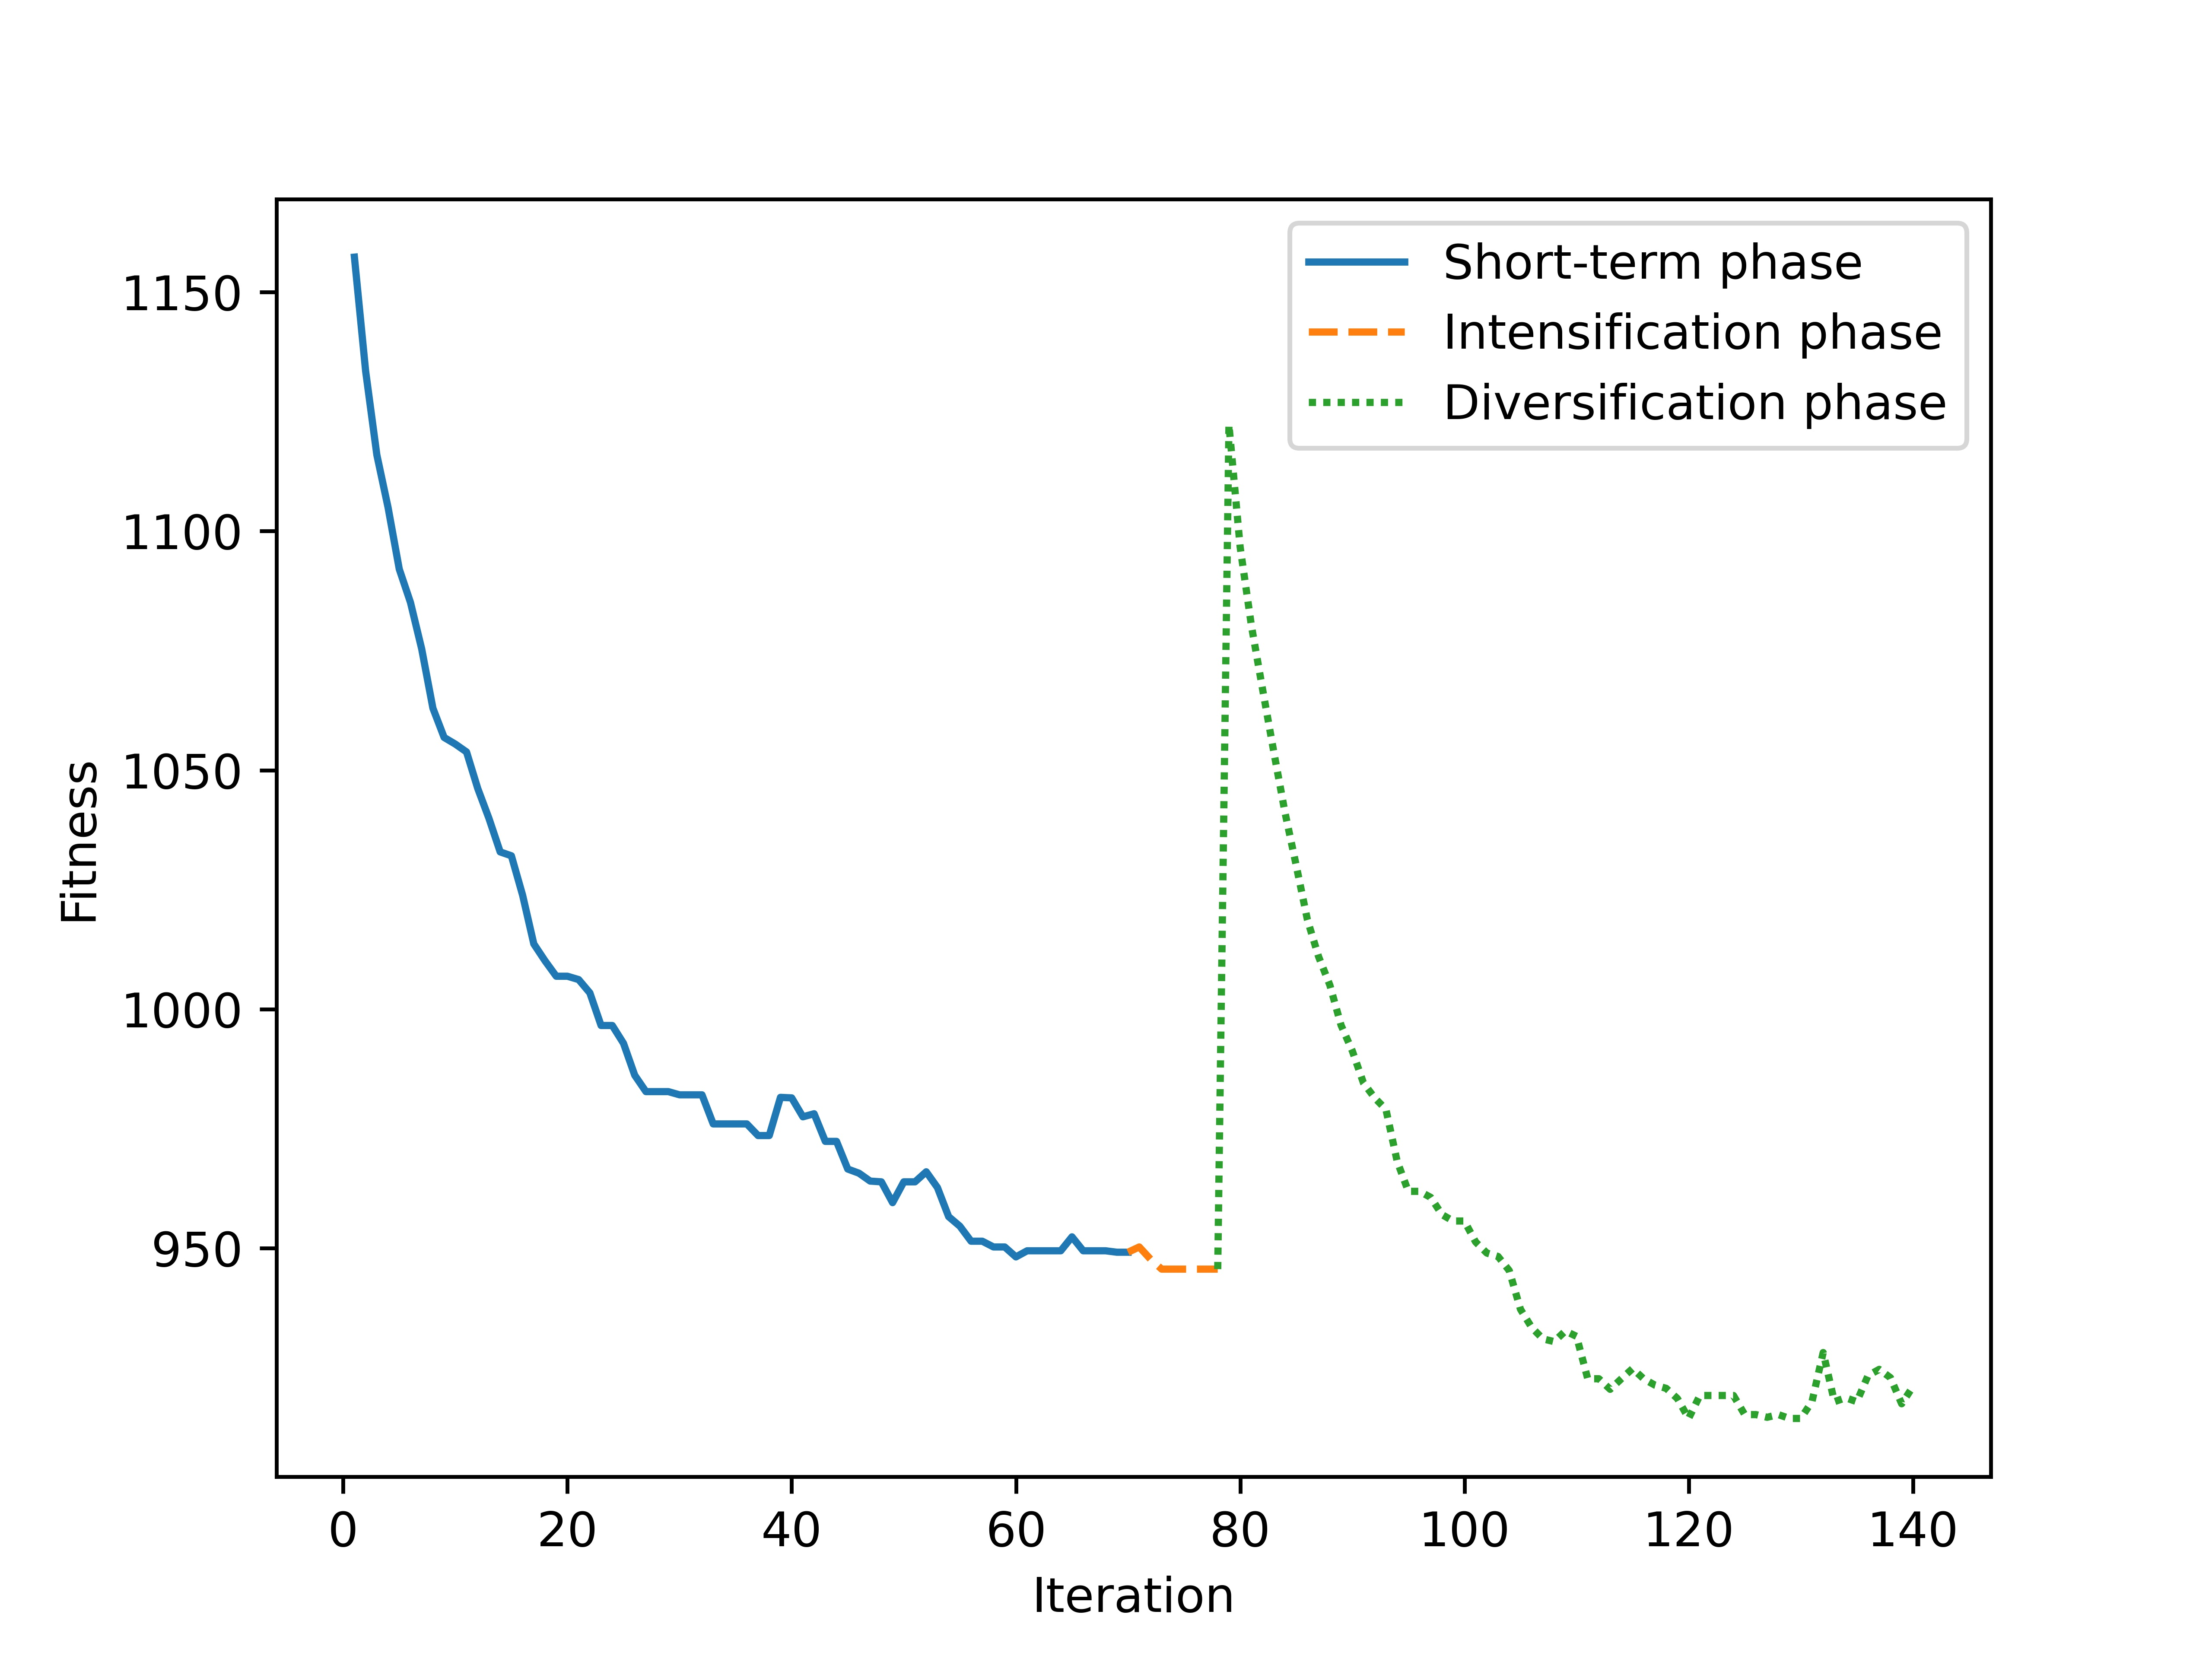
\includegraphics[width=0.95\textwidth]{images/converge_1.jpg}
        \caption{CMT07}
    \end{subfigure}
    \begin{subfigure}[b]{0.48\linewidth}
        \centering
        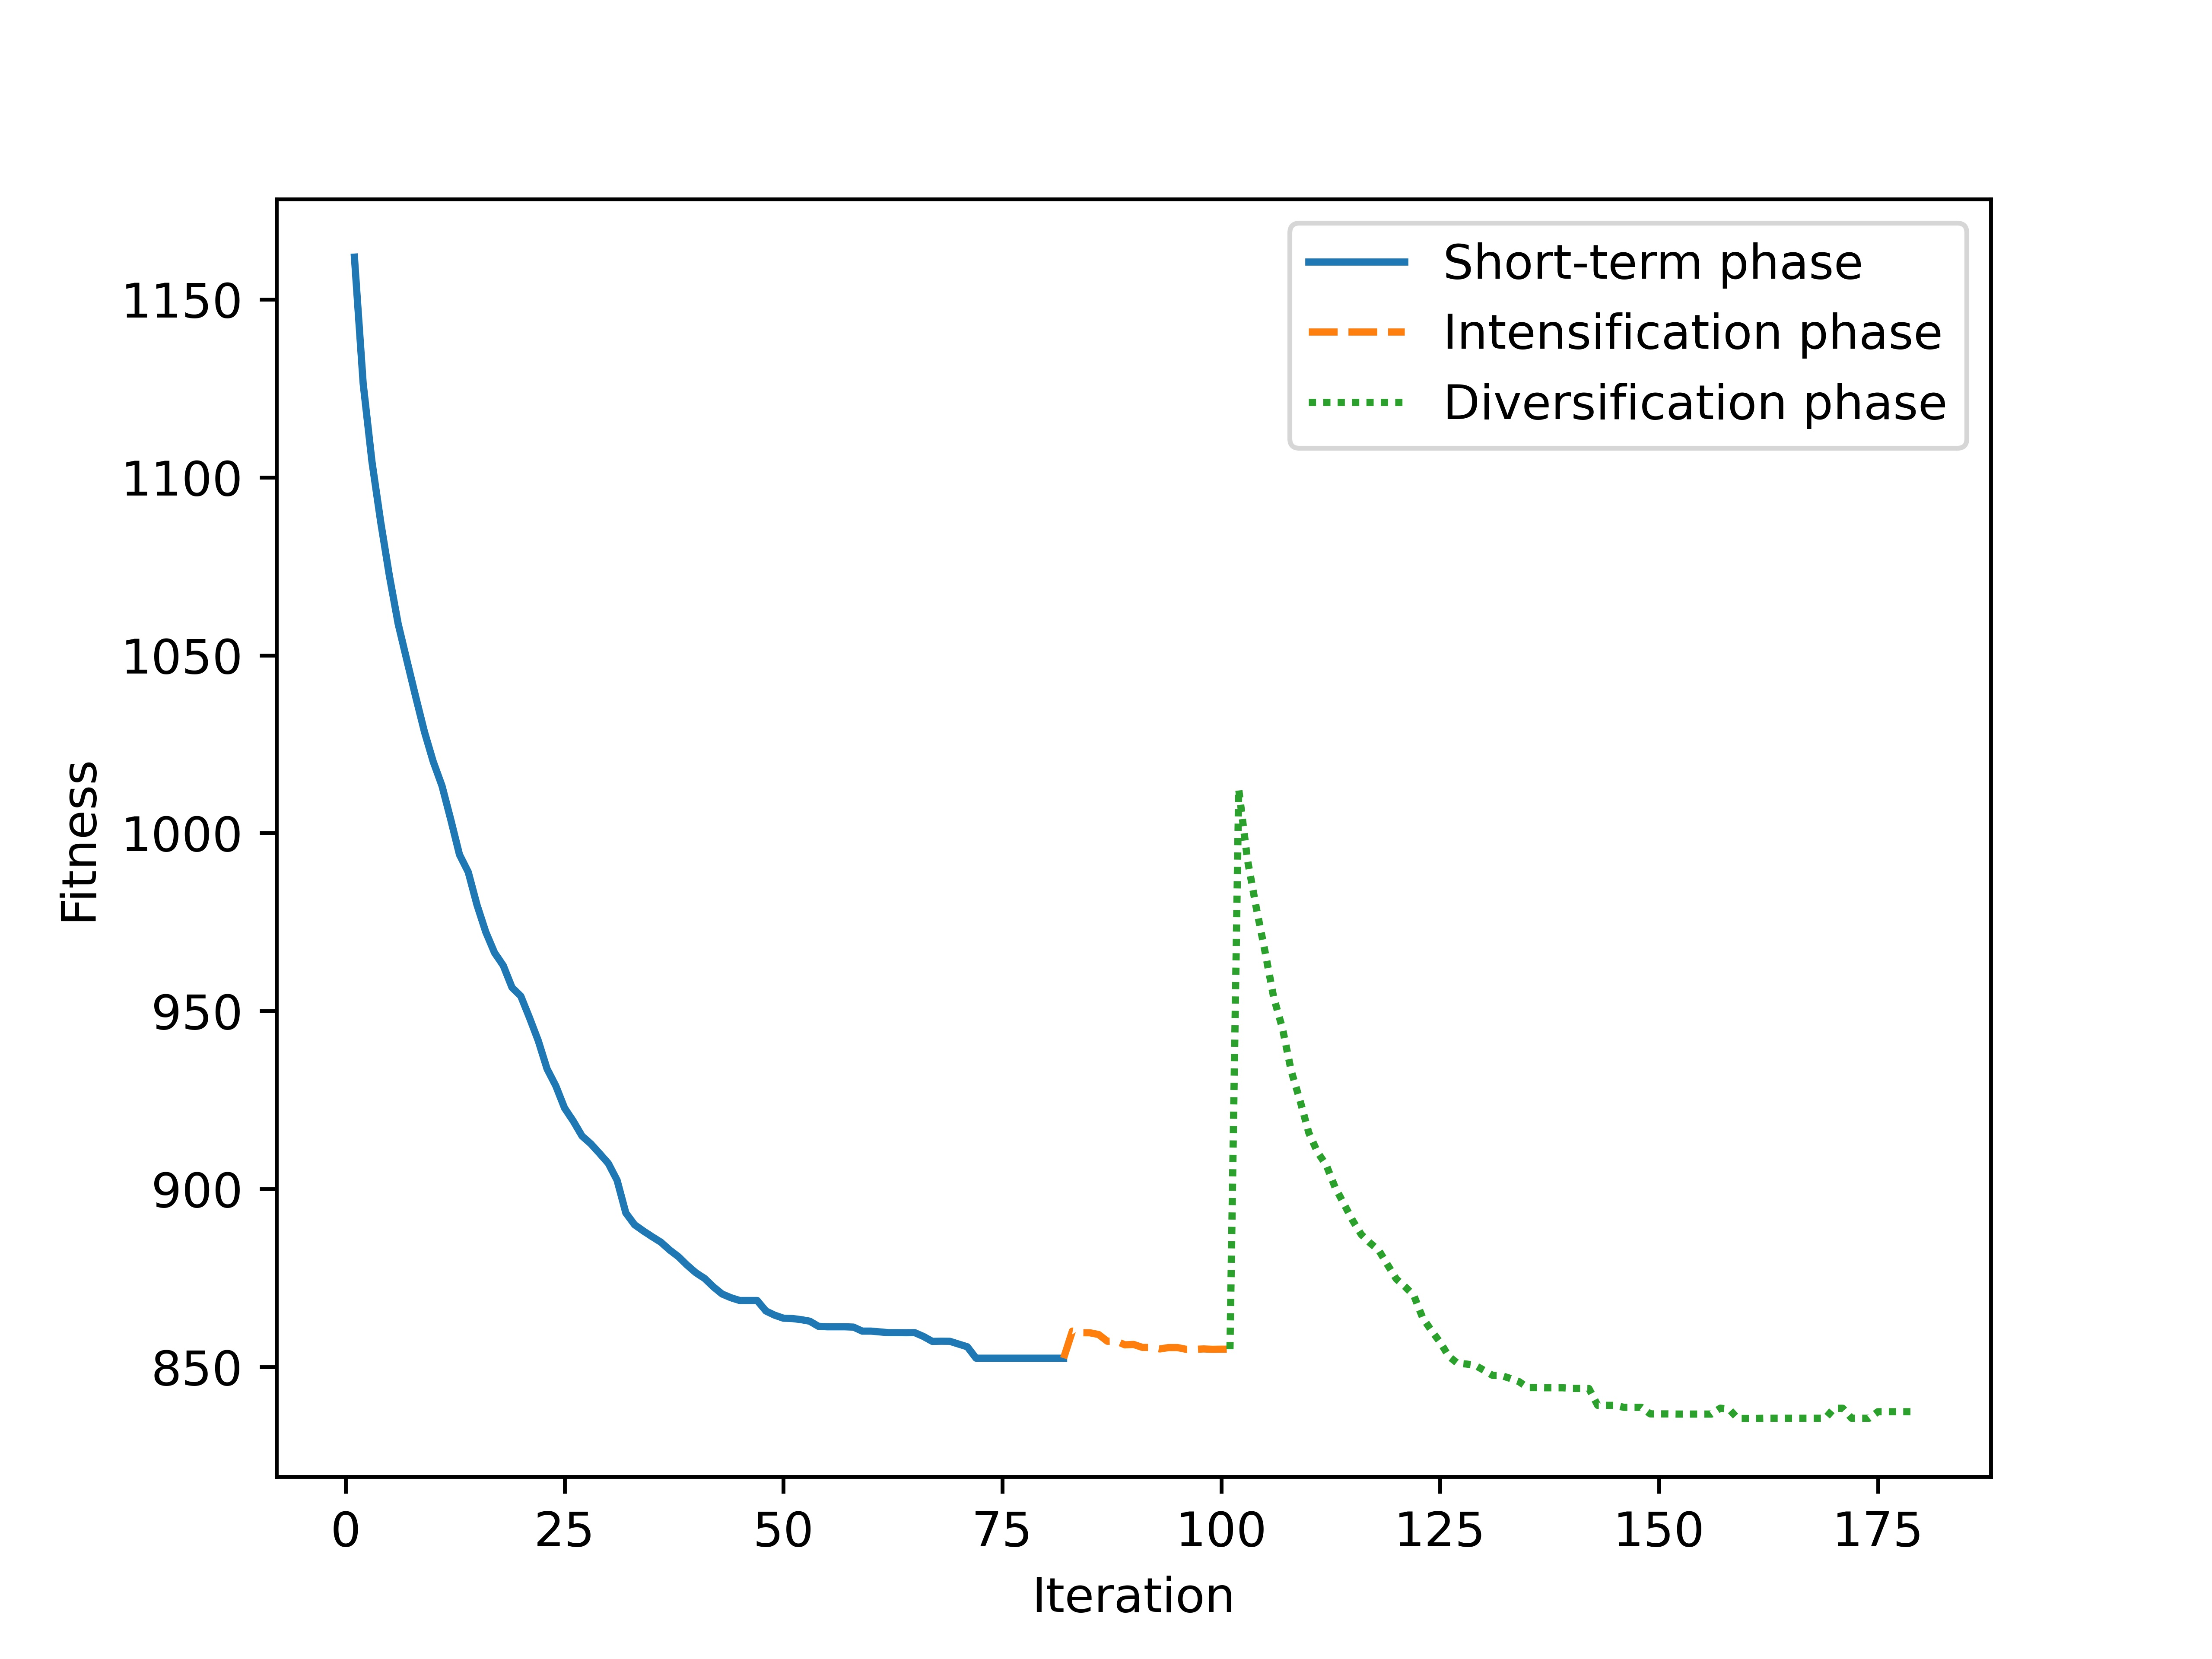
\includegraphics[width=0.95\textwidth]{images/converge_2.jpg}
        \caption{CMT12}
    \end{subfigure}
    \caption{Sample convergence charts for SimpleTabu}
\end{figure}
\end{frame}

\begin{frame}{Execution time}
\begin{figure}
    \centering
    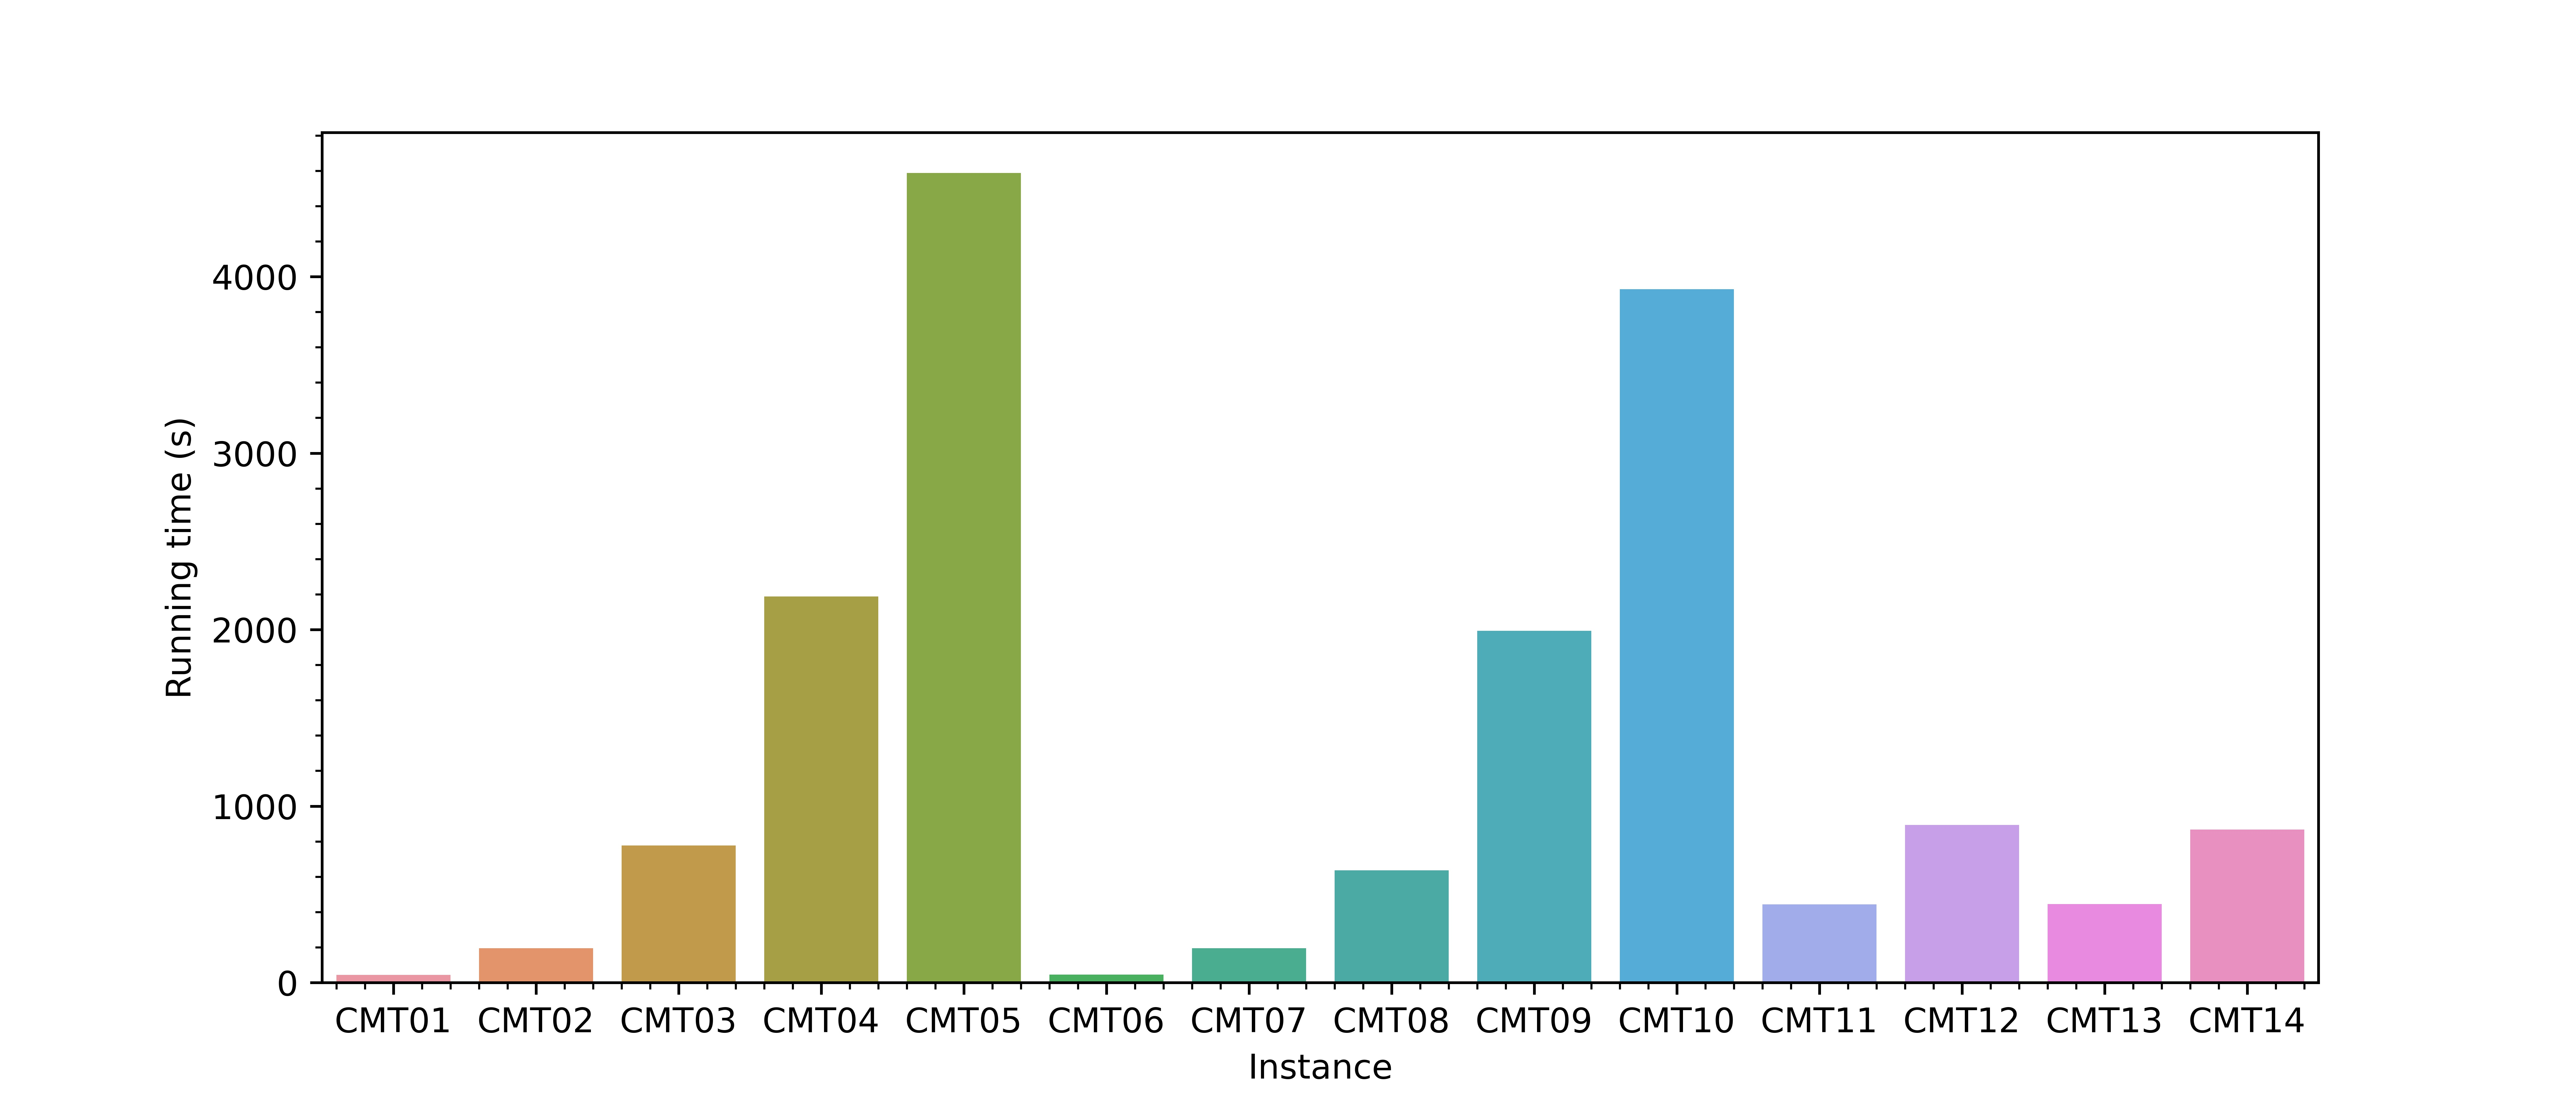
\includegraphics[width=\textwidth]{images/runtime_cmt.jpg}
    \caption{Average execution time over 5 runs for SimpleTabu on the Christofides 1979 dataset}
\end{figure}
\end{frame}

\section{Conclusions}
\begin{frame}{Conclusions}
Tabu search is a powerful metaheuristic for discrete optimization problems.
A simple implementation like SimpleTabu can still achieve competitive performance.

Selection of exploration operators is crucial for tabu search and local search in general.
\end{frame}

\begin{frame}{Thank you}
    \begin{center}
        \Huge{Thank you for listening!}
    \end{center}
\end{frame}

\begin{frame}[allowframebreaks]
    \frametitle{References}
    \bibliographystyle{plain}
    \bibliography{report.bib}
\end{frame}

\end{document}
